\documentclass[9pt, oneside]{amsart}   	
\usepackage{amssymb}
\usepackage{amsmath}
\usepackage{color}
\usepackage[usenames,dvipsnames,svgnames,table]{xcolor}
\usepackage[utf8]{inputenc}
\usepackage[colorlinks=true, pdfstartview=FitV,linkcolor=ForestGreen,citecolor=ForestGreen, urlcolor=black]{hyperref}
\usepackage{tikz}
\usetikzlibrary{patterns}
\usetikzlibrary{backgrounds}

\begin{document}

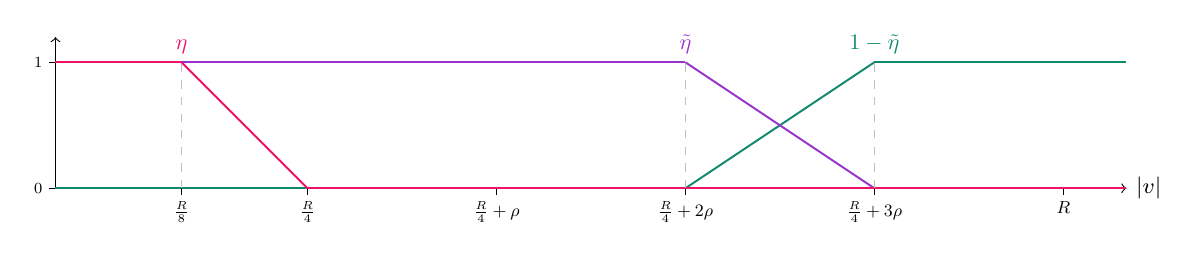
\begin{tikzpicture}[scale=1.6]
  % 1 on y axis
  \draw (-5,1) -- (-5.05, 1) node[anchor=east, scale =0.7] {\footnotesize{$1$}};
  % 0 on y axis
  \draw (-5,0) -- (-5.05, 0) node[anchor=east, scale =0.7] {\footnotesize{$0$}};
  % r/2 on x axis
  \draw (-4, 0) -- (-4, -0.05) node[anchor=north, scale =0.7] {\small$\frac{R}{8}$};
  % r on x axis
  \draw (-3, 0) -- (-3, -0.05) node[anchor=north, scale =0.7] {\small$\frac{R}{4}$};
  \draw (-1.5, 0) -- (-1.5, -0.05) node[anchor=north, scale =0.7] {\small$\frac{R}{4}+\rho$};
  \draw (0, 0) -- (0, -0.05) node[anchor=north, scale =0.7] {\small$\frac{R}{4}+2\rho$};
  \draw (1.5, 0) -- (1.5, -0.05) node[anchor=north, scale =0.7] {\small$\frac{R}{4}+3\rho$};
  % R on x axis
  \draw (3, 0) -- (3, -0.05) node[anchor=north, scale =0.7] {\small$R$};
  \draw[WildStrawberry, line width = 0.7pt](-5, 1) -- (-4, 1) node[anchor=south, scale =0.8] {$\eta$};
  \draw[WildStrawberry, line width = 0.7pt] (-4, 1) -- (-3, 0);
  \draw[WildStrawberry, line width = 0.7pt] (-3, 0) -- (3.5, 0);
  \begin{scope}[on background layer]
  %axes
    \draw[->] (-5, 0) -- (3.5, 0) node[right] {\footnotesize{$\vert v\vert $}};
  \draw[->] (-5, 0) -- (-5, 1.2);
  \draw[PineGreen, line width = 0.7pt] (-5, 0) -- (0, 0);
  \draw[PineGreen, line width = 0.7pt] (0, 0) -- (1.5, 1)node[anchor=south, scale =0.8] {$1-\tilde \eta$};
  \draw[PineGreen, line width = 0.7pt] (1.5, 1) -- (3.5,1);
  \draw[DarkOrchid, line width = 0.7pt] (-5, 1) -- (0, 1)node[anchor=south, scale =0.8] {$\tilde \eta$};
  \draw[DarkOrchid, line width = 0.7pt] (0, 1) -- (1.5, 0);
  \draw[DarkOrchid, line width = 0.7pt] (1.5, 0) -- (3.5,0);
  \end{scope}
  % aux lines
    \draw[lightgray, dashed] (-4, 0) -- (-4, 1);
  \draw[lightgray, dashed] (1.5, 0) -- (1.5, 1);
  \draw[lightgray, dashed] (0, 0) -- (0, 1);
\end{tikzpicture}

\end{document}